% !TEX encoding = UTF-8 Unicode

% Compilation using 'acmsmall.cls' - version 1.3 (March 2012), Aptara Inc.
% (c) 2010 Association for Computing Machinery (ACM)
%
% Questions/Suggestions/Feedback should be addressed to => "acmtexsupport@aptaracorp.com".
% Users can also go through the FAQs available on the journal's submission webpage.
%
% Steps to compile: latex, bibtex, latex, latex


\documentclass[prodmode,acmtochi]{acmsmall} % Aptara syntax

% Package to generate and customize Algorithm as per ACM style
\usepackage[ruled]{algorithm2e}
\renewcommand{\algorithmcfname}{ALGORITHM}
\SetAlFnt{\small}
\SetAlCapFnt{\small}
\SetAlCapNameFnt{\small}
\SetAlCapHSkip{0pt}
\IncMargin{-\parindent}

% Packages
\usepackage[super]{nth}
\usepackage[inline]{enumitem}
\usepackage{moreenum}
\usepackage{tabu}
\usepackage{booktabs}
\usepackage{array}
\newcommand{\ra}[1]{\renewcommand{\arraystretch}{#1}}
\newcommand{\urlhttp}[1]{\href{http://#1}{\nolinkurl{#1}}}
\newcommand{\urlhttps}[1]{\href{https://#1}{\nolinkurl{#1}}}

% Metadata Information
\acmVolume{9}
\acmNumber{4}
\acmArticle{39}
\acmYear{2010}
\acmMonth{3}

% Copyright
%\setcopyright{acmcopyright}
%\setcopyright{acmlicensed}
%\setcopyright{rightsretained}
%\setcopyright{usgov}
%\setcopyright{usgovmixed}
%\setcopyright{cagov}
%\setcopyright{cagovmixed}

% DOI
\doi{0000001.0000001}

%ISSN
\issn{1234-56789}

% Document starts
\begin{document}

% Page heads
\markboth{B. Harmon et al.}{Embodied Spatial Cognition in Tangible Computing}

% Title portion
\title{Embodied Spatial Cognition in Tangible Computing} % Spatial Performance in Tangible Computing 
\author{BRENDAN ALEXANDER HARMON
\affil{North Carolina State University}
ANNA PETRASOVA
\affil{North Carolina State University}
VACLAV PETRAS
\affil{North Carolina State University}
HELENA MITASOVA
\affil{North Carolina State University}
ROSS ​KENDALL MEENTEMEYER
\affil{North Carolina State University}
EUGENE BRESSLER
\affil{North Carolina State University}
ART RICE
\affil{North Carolina State University}}

\begin{abstract}
%
\end{abstract}

%
% The code below should be generated by the tool at
% http://dl.acm.org/ccs.cfm
% Please copy and paste the code instead of the example below. 
%
\begin{CCSXML}
<ccs2012>
<concept>
<concept_id>10003120.10003121</concept_id>
<concept_desc>Human-centered computing~Human computer interaction (HCI)</concept_desc>
<concept_significance>500</concept_significance>
</concept>
<concept>
<concept_id>10003120.10003121.10003122.10011749</concept_id>
<concept_desc>Human-centered computing~Laboratory experiments</concept_desc>
<concept_significance>500</concept_significance>
</concept>
</ccs2012>
\end{CCSXML}

\ccsdesc[500]{Human-centered computing~Human computer interaction (HCI)}
\ccsdesc[500]{Human-centered computing~Laboratory experiments}
%
% End generated code
%

\keywords{Human-computer interaction, tangible interfaces, interaction design, physical computation, embodied cognition, spatial thinking, geospatial modeling}

\acmformat{Brendan A. Harmon, Anna Petrasova, Vaclav Petras, Helena Mitasova, Ross K. Meentemeyer, Eugene H. Bressler, and Art Rice, 2016. Embodied Spatial Cognition in Tangible Computing.}

\begin{bottomstuff}
Author's addresses: B. A. Harmon {and} A. Petrasova {and} V. Petras {and} H. Mitasova {and} R. K. Meentemeyer, Center for Geospatial Analytics, North Carolina State University; B. A. Harmon, E. H. Bressler {and} A. Rice, Department of Landscape Architecture, North Carolina State University.
\end{bottomstuff}


\maketitle

\pagebreak

\section{Figures}

\begin{figure*}[h!]
\begin{center}
		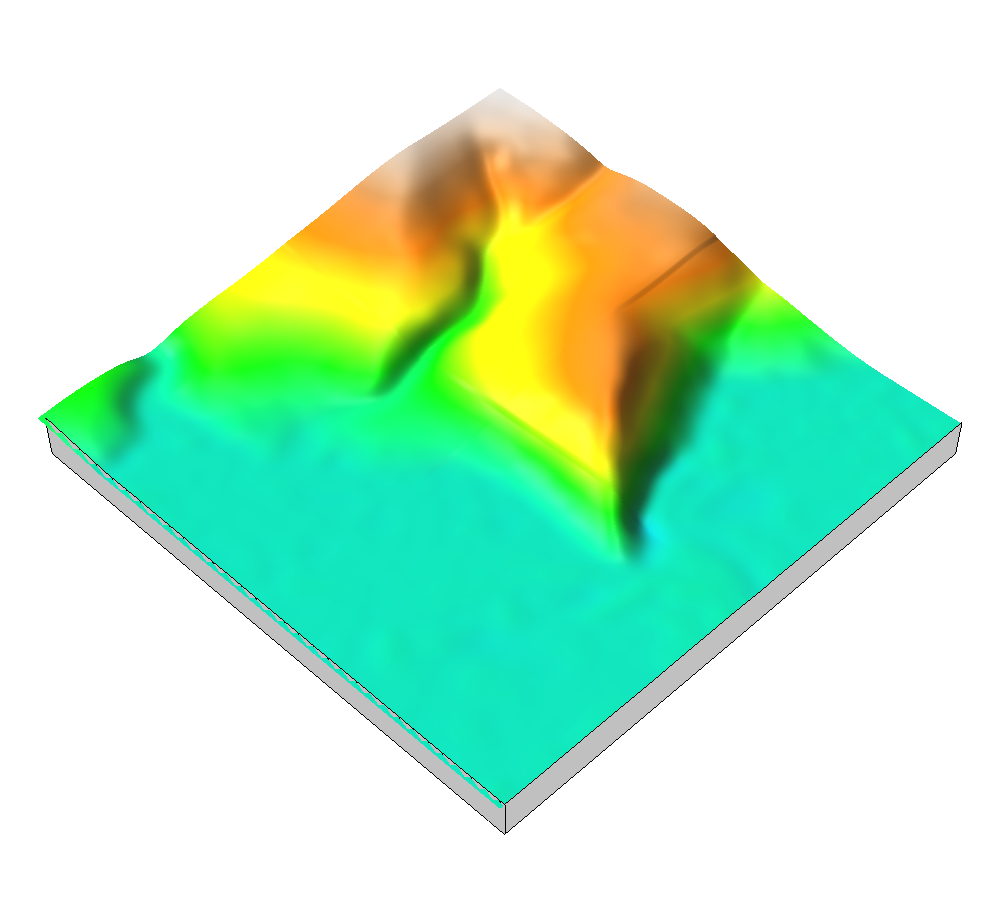
\includegraphics[width=0.32\textwidth]{images/bivariate_scatterplots/dem_1.png}
		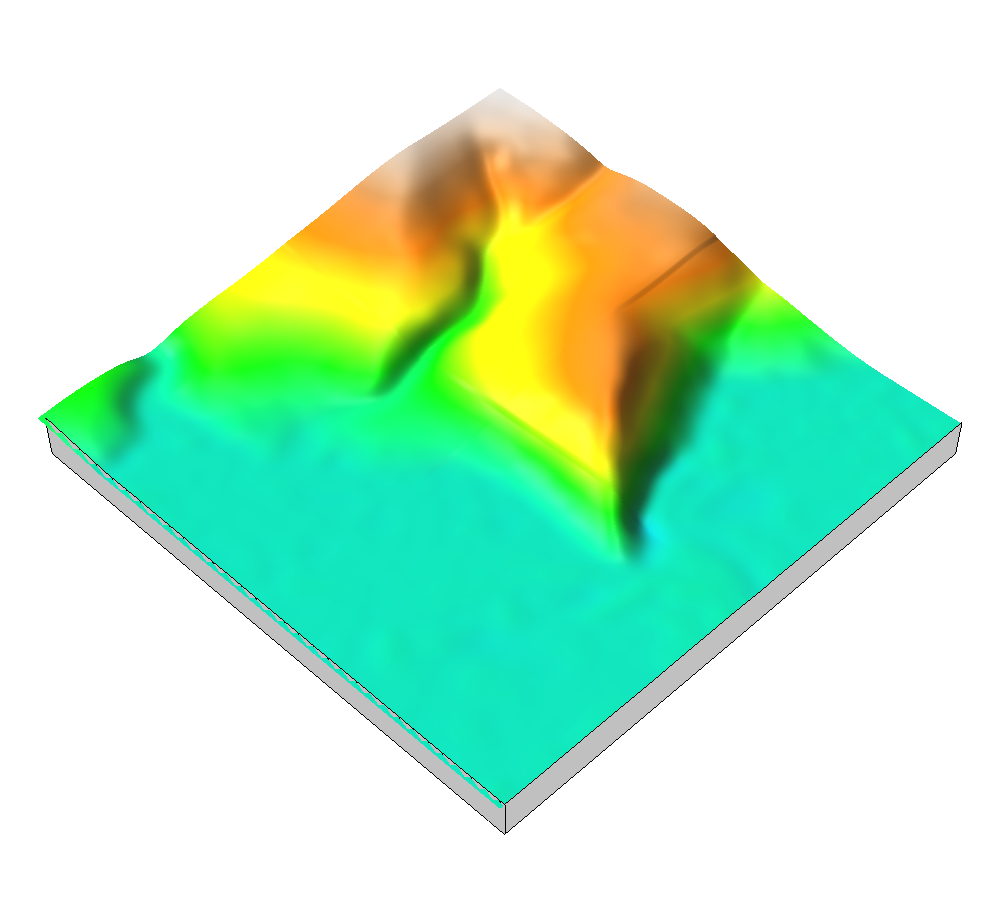
\includegraphics[width=0.32\textwidth]{images/bivariate_scatterplots/dem_2.png}
		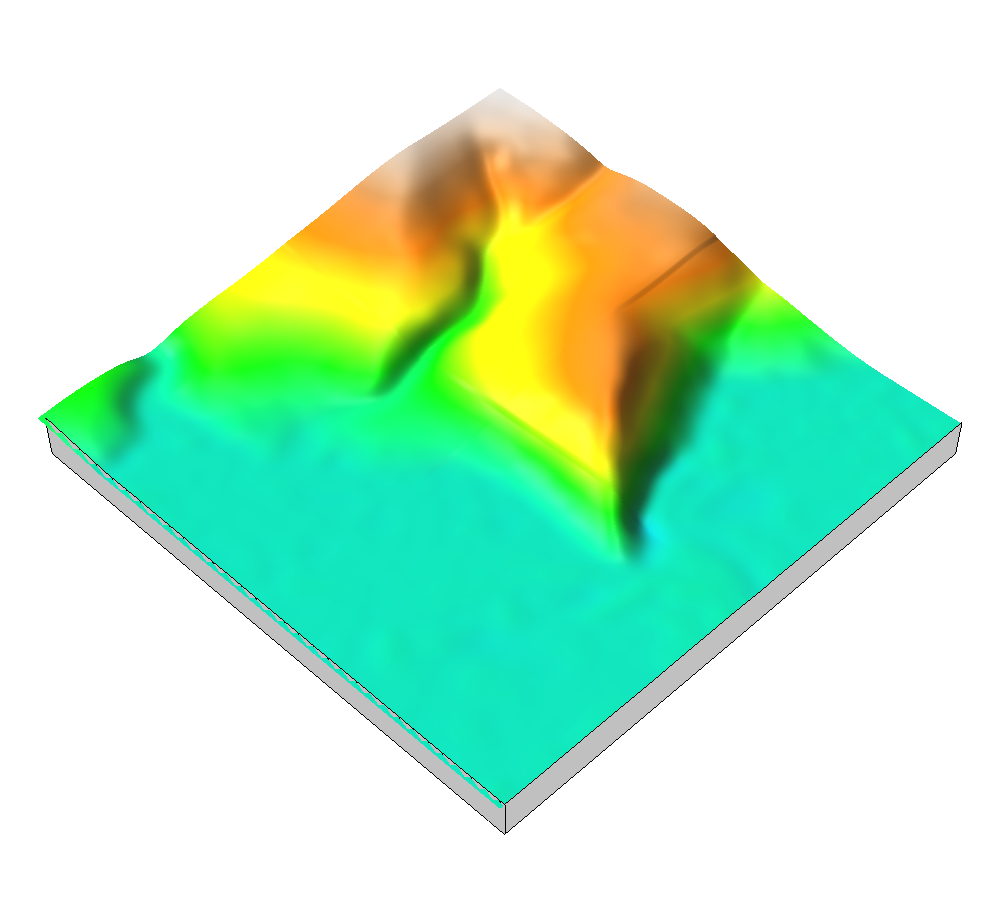
\includegraphics[width=0.32\textwidth]{images/bivariate_scatterplots/dem_3.png}
	\caption{Bivariate scatterplots}
	\label{fig:scatterplots}
\end{center}
\end{figure*}

\begin{figure*}[h!]
\begin{center}
		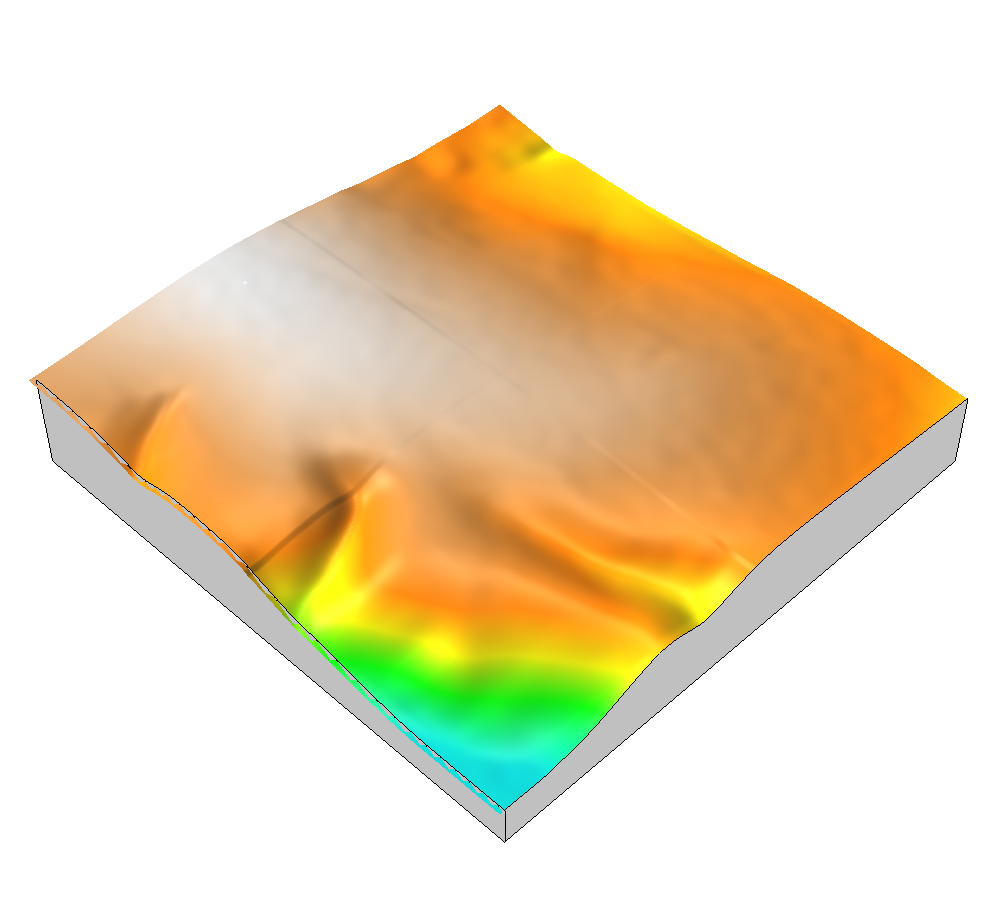
\includegraphics[width=0.32\textwidth]{images/bivariate_scatterplots/dem_4.png}
		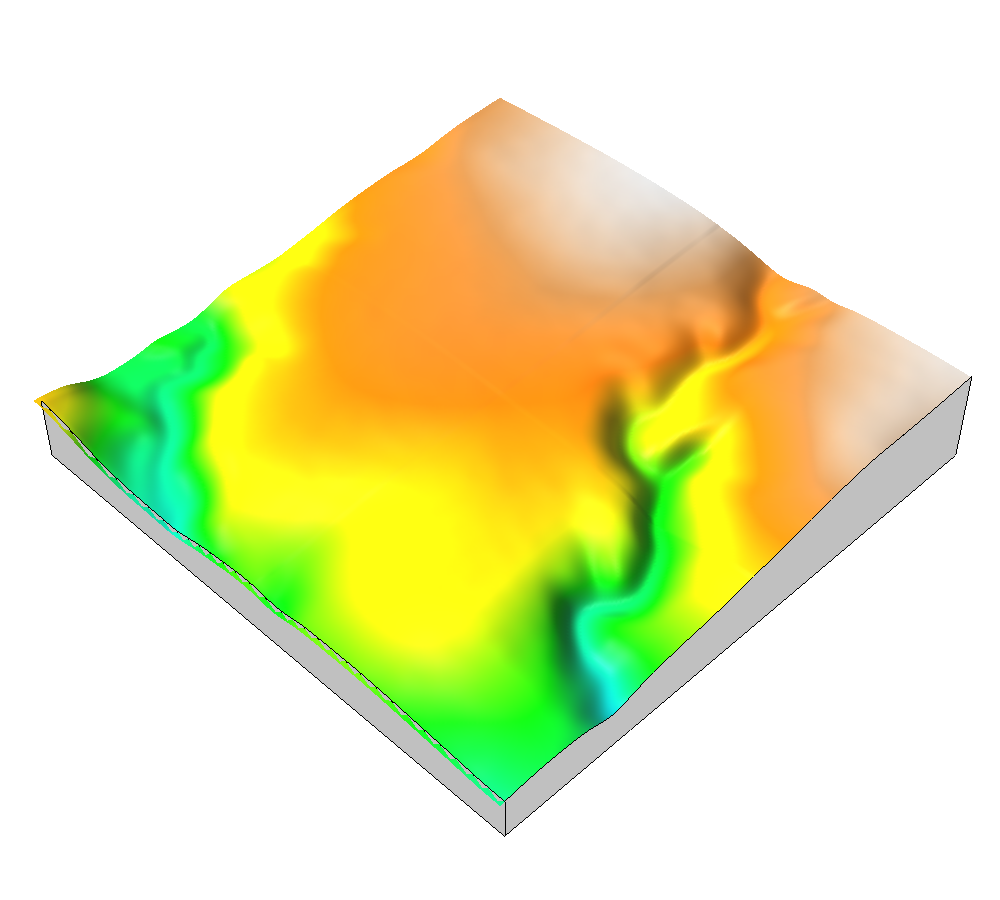
\includegraphics[width=0.32\textwidth]{images/bivariate_scatterplots/dem_5.png}
	\caption{Bivariate scatterplots}
	\label{fig:scatterplots}
\end{center}
\end{figure*}

\pagebreak

%%%%%%%%%%%%%%%%%%  SCATTERPLOT TABLE

\begin{table}
\tbl{Bivariate scatterplots of elevation values}{
\ra{1.3}
\begin{tabular}{m{0.1\textwidth} m{0.32\textwidth} m{0.32\textwidth} m{0.32\textwidth}}
\toprule
& \multicolumn{1}{c}{Digital} & \multicolumn{1}{c}{Analog}  & \multicolumn{1}{c}{Augmented}\\
\midrule \\
Mean & 
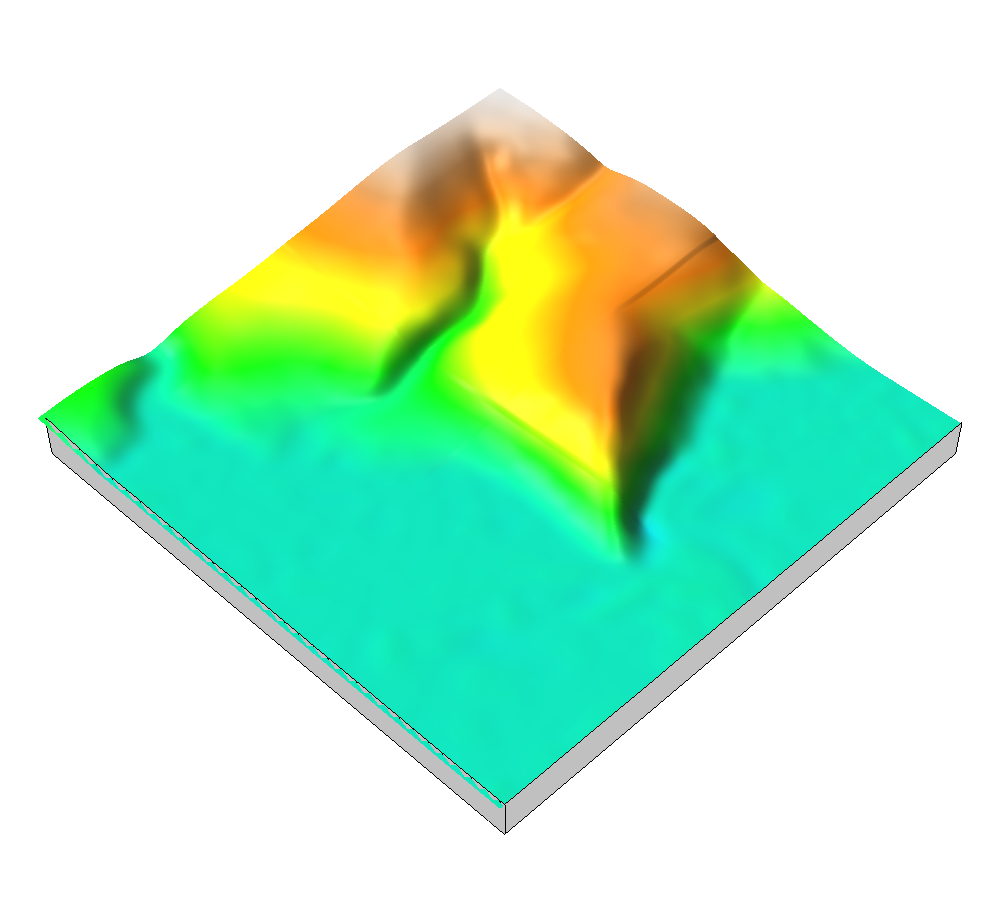
\includegraphics[width=0.32\textwidth]{images/bivariate_scatterplots/dem_1.png} &
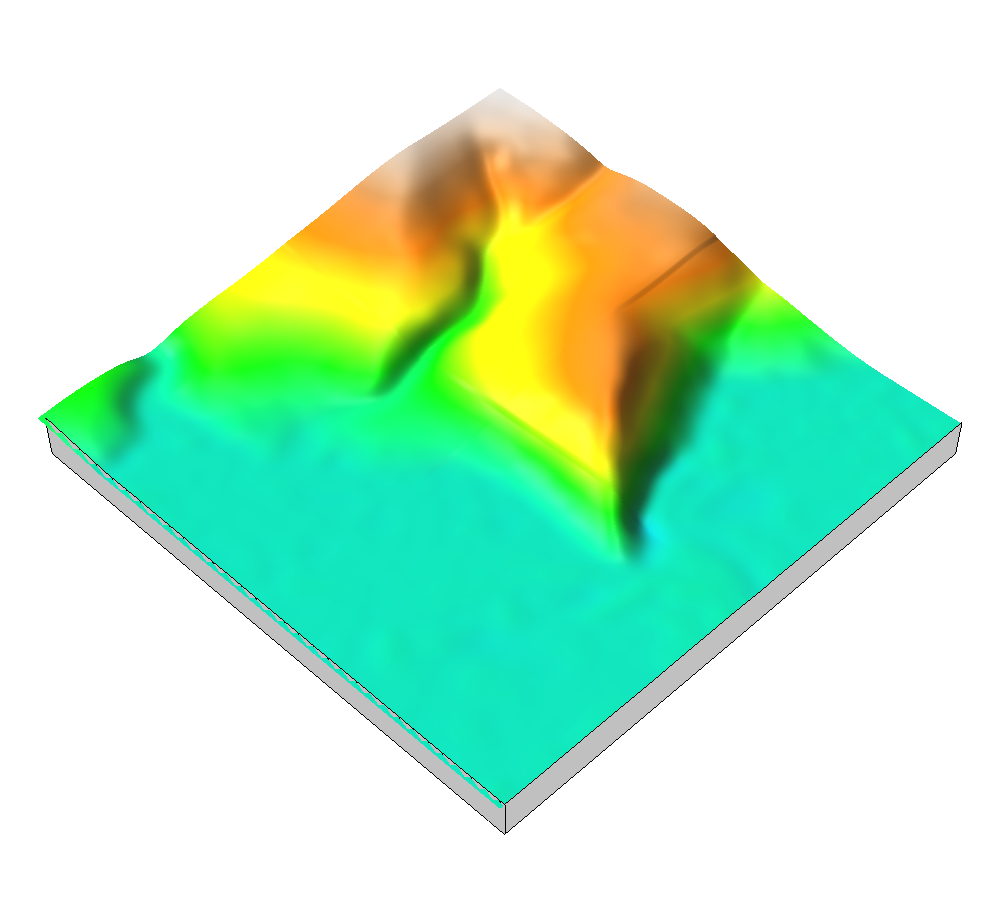
\includegraphics[width=0.32\textwidth]{images/bivariate_scatterplots/dem_2.png} &
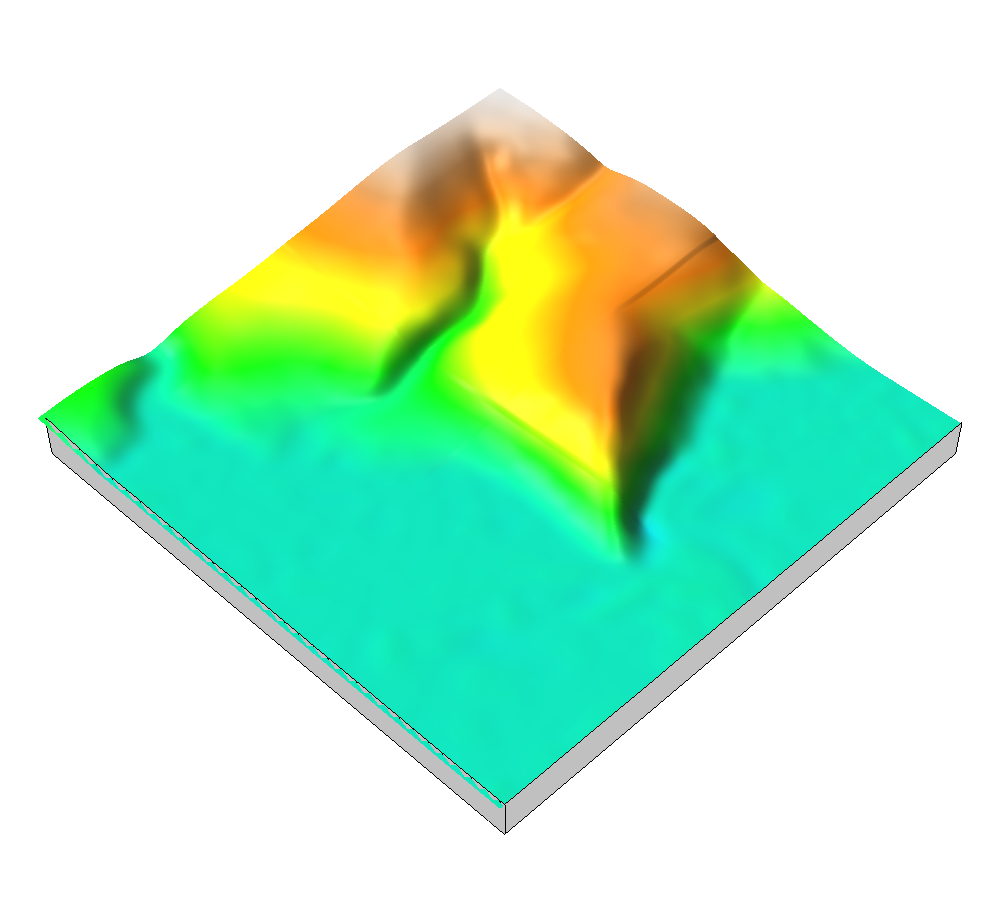
\includegraphics[width=0.32\textwidth]{images/bivariate_scatterplots/dem_3.png}\\
& \multicolumn{1}{c}{Reference} & \multicolumn{1}{c}{Reference} & \multicolumn{1}{c}{Reference} \\
\\
\bottomrule
\end{tabular}}
\label{table:scatterplots} 
\end{table}



\end{document}



